%%========================================================================
%% LaTeX sjabloon voor bachelorproef toegepaste informatica
%%  HoGent Bedrijf en Organisatie - Bijlagenbundel
%%========================================================================

%%========================================================================
%% Preamble
%%========================================================================

\documentclass[pdftex,a4paper,12pt,twoside]{report}

% XXX: Let op: dit sjabloon is gemaakt om dubbelzijdig af te drukken
% Voor enkelzijdig, verwijder ``twoside'' hierboven.

%%---------- Extra functionaliteit ---------------------------------------

\usepackage[utf8]{inputenc}  % Accenten gebruiken in tekst (vb. é ipv \'e)
\usepackage{amsfonts}        % AMS math packages: extra wiskundige
\usepackage{amsmath}         %   symbolen (o.a. getallen-
\usepackage{amssymb}         %   verzamelingen N, R, Z, Q, etc.)
\usepackage[english]{babel}    % Taalinstellingen: woordsplitsingen,
                             %  commando's voor speciale karakters
                             %  ("english" voor ENG)
\usepackage{eurosym}         % Euro-symbool €
\usepackage{geometry}
\usepackage{graphicx}        % Invoegen van tekeningen
\usepackage[pdftex,bookmarks=true]{hyperref}
                             % PDF krijgt klikbare links & verwijzingen,
                             %  inhoudstafel
\usepackage{listings}        % Broncode mooi opmaken
\usepackage{multirow}        % Tekst over verschillende cellen in tabellen
\usepackage{rotating}        % Tabellen en figuren roteren
\usepackage{natbib}          % Betere bibliografiestijlen
\usepackage{fancyhdr}        % Pagina-opmaak met hoofd- en voettekst

\usepackage[T1]{fontenc}     % Ivm lettertypes
\usepackage{lmodern}
\usepackage{textcomp}

\usepackage{pgfplots}
\usepackage[toc,page]{appendix}

\usepackage{lipsum}          % Voor vultekst (lorem ipsum)

%%---------- Layout ------------------------------------------------------

% hoofdingen, enz.
\pagestyle{fancy}
% enkel hoofdstuktitel in hoofding, geen sectietitel (vermijd overlap)
\renewcommand{\sectionmark}[1]{}

% lijn, wordt gebruikt in titelpagina
\newcommand{\HRule}{\rule{\linewidth}{0.5mm}}

% Leeg blad
\newcommand{\emptypage}{
\newpage
\thispagestyle{empty}
\mbox{}
\newpage
}

% Gebruik een schreefloos lettertype ipv het "oubollig" uitziende
% Computer Modern
\renewcommand{\familydefault}{\sfdefault}

% Commando voor invoegen Java-broncodebestanden (dank aan Niels Corneille)
% Gebruik: \javacode{source/MijnKlasse.java}{Uitleg bij de code}
\newcommand{\javacode}[2]{ \lstset{%
  language=java,
  breaklines=true,
  float=th,
  caption={#2},
  basicstyle=\scriptsize,
  frame=single,
  extendedchars=\true
}
\lstinputlisting{#1}}

%%---------- Documenteigenschappen ---------------------------------------
%% Vul dit aan met je eigen info:

% Je eigen naam
\newcommand{\student}{Frederik De Smedt}

% De naam van je lector, begeleider, promotor
\newcommand{\promotor}{Joeri Van Herreweghe}

% De naam van je co-promotor
\newcommand{\copromotor}{Jens Buysse}

% Indien je bachelorproef in opdracht van een bedrijf of organisatie
% geschreven is, geef je hier de naam.
\newcommand{\instelling}{---}

% De titel van het rapport/bachelorproef
\newcommand{\titel}{Research of caching strategies in mobile native applications using external data services}

% Datum van indienen
\newcommand{\datum}{29 mei 2015}

% Faculteit
\newcommand{\faculteit}{Faculty Business \& Information Management}

% Soort rapport
\newcommand{\rapporttype}{Bachelor's thesis submitted to achieve the degree of\\Bachelor in the Applied Computer Science}

% Academiejaar
\newcommand{\academiejaar}{2015-2016}

% Examenperiode
%  - 1e semester = 1e examenperiode
%  - 2e semester = 2e examenperiode
%  - tweede zit = 3e examenperiode
\newcommand{\examenperiode}{Examination period 2}

\newcommand{\RuntimeGraphLarge}[2]{
\pgfplotsset{width=7cm,compat=1.13}
\begin{tikzpicture}
\begin{axis}[
	title=#1, 
	xlabel={Cache size}, 
	ylabel={Avg runtime (ns)},
	ymin=0, ymax=#2,
]
\addplot table {Data/#1.dat};
\end{axis}
\end{tikzpicture}
}

\newcommand{\codefragment}[2]{ \lstset{%
  language=java,
  breaklines=true,
  float=th,
  caption={#2},
  basicstyle=\scriptsize,
  frame=single,
  extendedchars=\true
}
\lstinputlisting{#1}}

\newcommand{\RuntimeGraph}[1]{
\pgfplotsset{width=7cm,compat=1.13}
\begin{tikzpicture}
\begin{axis}[
	title=#1, 
	xlabel={Cache ratio}, 
	ylabel={Avg runtime (ns)},
	ymin=0, ymax=5000,
]
\addplot table {Data/#1.dat};
\end{axis}
\end{tikzpicture}
}

\newcommand{\RHitGraph}[1]{
\pgfplotsset{width=12cm,compat=1.13,height=9cm}
\begin{tikzpicture}
\begin{axis}[
	title=#1, 
	xlabel={Cached ratio (\%)}, 
	ylabel={Hit ratio (\%)},
	ymin=0, ymax=100,
	legend entries={NFS,Web12,Zipf,Random},
	legend pos=outer north east,
	legend cell align=left
]
\addplot table[
	x={Cache_ratio},
	y=NFS
] {Data/#1HitRatio.dat};
\addplot table[
	x={Cache_ratio},
	y=Web12
] {Data/#1HitRatio.dat};
\addplot table[
	x={Cache_ratio},
	y=Zipf
] {Data/#1HitRatio.dat};
\addplot table[
	x={Cache_ratio},
	y=Random
] {Data/#1HitRatio.dat};

\end{axis}
\end{tikzpicture}
}

\newcommand{\RHitGraphTrace}[3]{
\pgfplotsset{width=12cm,compat=1.13,height=18cm}
\begin{tikzpicture}
\begin{axis}[
	title=#1, 
	xlabel={Cached ratio (\%)}, 
	ylabel={Hit ratio (\%)},
	ymin=#2, ymax=#3,
	legend entries={ARC,CLOCK,Guava,Random,NLRU,FIFO,LIRS},
	legend pos=outer north east,
	legend cell align=left
]
\addplot table[
	x={Cache_ratio},
	y=ARC
] {Data/#1HitRatio.dat};
\addplot table[
	x={Cache_ratio},
	y=CLOCK
] {Data/#1HitRatio.dat};
\addplot table[
	x={Cache_ratio},
	y=Guava
] {Data/#1HitRatio.dat};
\addplot table[
	x={Cache_ratio},
	y=Random
] {Data/#1HitRatio.dat};
\addplot table[
	x={Cache_ratio},
	y=NLRU
] {Data/#1HitRatio.dat};
\addplot table[
	x={Cache_ratio},
	y=FIFO
] {Data/#1HitRatio.dat};
\addplot table[
	x={Cache_ratio},
	y=LIRS
] {Data/#1HitRatio.dat};

\end{axis}
\end{tikzpicture}
}

\newcommand{\RRuntimeGraphTrace}[3]{
\pgfplotsset{width=12cm,compat=1.13,height=18cm}
\begin{tikzpicture}
\begin{axis}[
	title=#1, 
	xlabel={Cached ratio (\%)}, 
	ylabel={Avg runtime (ns)},
	ymin=#2, ymax=#3,
	legend entries={ARC,CLOCK,Guava,Random,NLRU,FIFO,LIRS},
	legend pos=outer north east,
	legend cell align=left
]
\addplot table[
	x={Cache_ratio},
	y=ARC
] {Data/#1AvgRuntime.dat};
\addplot table[
	x={Cache_ratio},
	y=CLOCK
] {Data/#1AvgRuntime.dat};
\addplot table[
	x={Cache_ratio},
	y=Guava
] {Data/#1AvgRuntime.dat};
\addplot table[
	x={Cache_ratio},
	y=Random
] {Data/#1AvgRuntime.dat};
\addplot table[
	x={Cache_ratio},
	y=NLRU
] {Data/#1AvgRuntime.dat};
\addplot table[
	x={Cache_ratio},
	y=FIFO
] {Data/#1AvgRuntime.dat};
\addplot table[
	x={Cache_ratio},
	y=LIRS
] {Data/#1AvgRuntime.dat};

\end{axis}
\end{tikzpicture}
}

\newcommand{\RAvgRuntimeGraph}[1]{
\pgfplotsset{width=12cm,compat=1.13,height=9cm}
\begin{tikzpicture}
\begin{axis}[
	title=#1, 
	xlabel={Cached ratio (\%)}, 
	ylabel={Avg runtime (ns)},
	ymin=0, ymax=7000,
	legend entries={NFS,Web12,Zipf,Random},
	legend pos=outer north east,
	legend cell align=left
]
\addplot table[
	x={Cache_ratio},
	y=NFS
] {Data/#1AvgTime.dat};
\addplot table[
	x={Cache_ratio},
	y=Web12
] {Data/#1AvgTime.dat};
\addplot table[
	x={Cache_ratio},
	y=Zipf
] {Data/#1AvgTime.dat};
\addplot table[
	x={Cache_ratio},
	y=Random
] {Data/#1AvgTime.dat};

\end{axis}
\end{tikzpicture}
}

%%========================================================================
%% Inhoud document
%%========================================================================

\begin{document}

%%---------- Front matter ------------------------------------------------
%% Het voorblad - Hier moet je in principe niets wijzigen.

\begin{titlepage}
  \newgeometry{top=2cm,bottom=1.5cm,left=1.5cm,right=1.5cm}
  \begin{center}

    \begingroup
    \rmfamily
    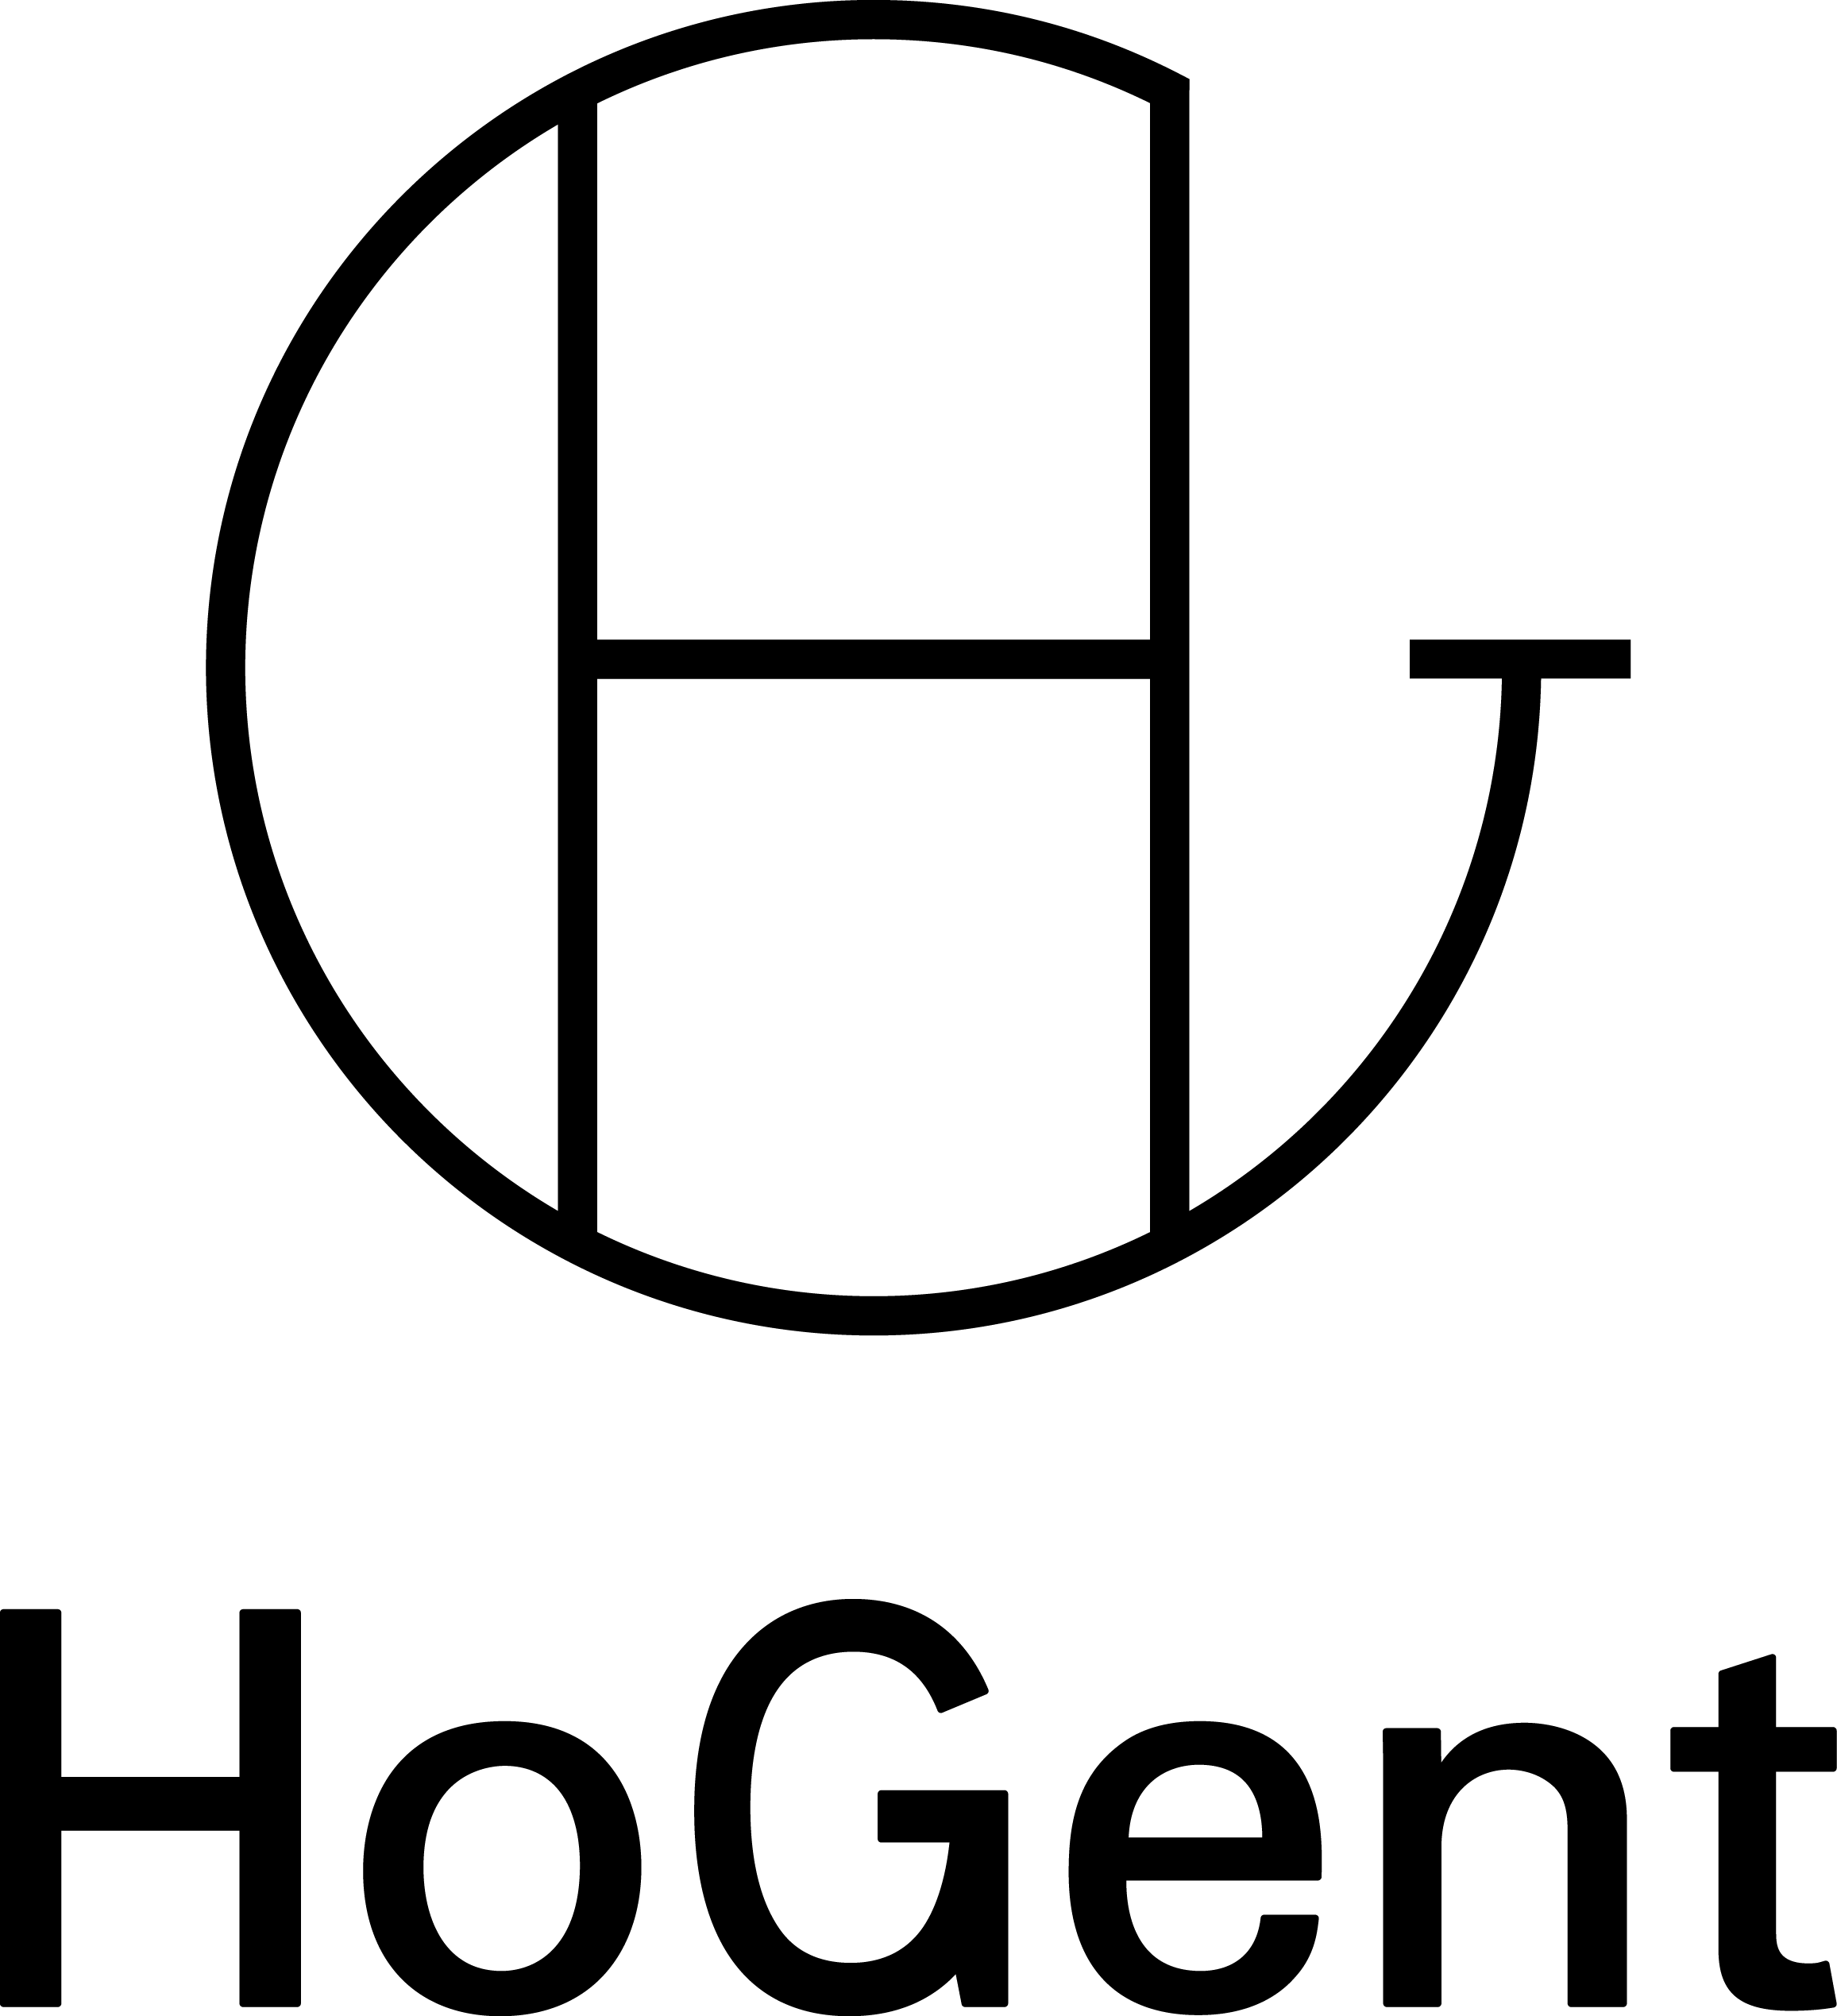
\includegraphics[width=2.5cm]{img/HG-beeldmerk-woordmerk}\\[.5cm]
    \faculteit\\[3cm]
    \titel\\[1cm]
    Appendix
    \vfill
    \student\\[3.5cm]
    \rapporttype\\[2cm]
    Supervisor:\\
    \promotor\\
    Co-supervisor:\\
    \copromotor\\[2.5cm]
    Organization: \instelling\\[.5cm]
    Academic year: \academiejaar\\[.5cm]
    \examenperiode
    \endgroup

  \end{center}
  \restoregeometry
\end{titlepage}

% Schutblad

\emptypage


\begin{titlepage}
  \newgeometry{top=5.35cm,bottom=1.5cm,left=1.5cm,right=1.5cm}
  \begin{center}

    \begingroup
    \rmfamily
    \faculteit\\[3cm]
    \titel\\[1cm]
    Appendix
    \vfill
    \student\\[3.5cm]
    \rapporttype\\[2cm]
    Supervisor:\\
    \promotor\\
    Co-supervisor:\\
    \copromotor\\[2.5cm]
    Organization: \instelling\\[.5cm]
    Academic year: \academiejaar\\[.5cm]
    \examenperiode
    \endgroup

  \end{center}
  \restoregeometry
\end{titlepage}


\tableofcontents
\newpage

\begin{appendices}
\chapter{Insert benchmarks}
\RuntimeGraph{RandomCacheInsert}
\RuntimeGraph{LIRSCacheInsert}
\RuntimeGraph{GuavaCacheInsert}
\RuntimeGraph{NativeLruCacheInsert}
\\\RuntimeGraph{FifoCacheInsert}
\\\\These benchmarks have an average execution time above 5000 ns. Due to the scale difference they are placed separately.
\\\\\RuntimeGraphLarge{ClockCacheInsert}{15000}
\RuntimeGraphLarge{ArcCacheInsert}{15000}

\chapter{Update benchmarks}

\RuntimeGraphLarge{LIRSCacheUpdate}{15000}
\RuntimeGraphLarge{GuavaCacheUpdate}{15000}
\\\RuntimeGraphLarge{NativeLruCacheUpdate}{15000}
\RuntimeGraphLarge{FifoCacheUpdate}{15000}
\\\RuntimeGraphLarge{ClockCacheUpdate}{15000}
\\\\Due to high average runtimes of ARC and random cache, they are placed separately and each have a different scale.
\\\\\RuntimeGraphLarge{ArcCacheUpdate}{20000}
\RuntimeGraphLarge{RandomCacheUpdate}{30000}

\chapter{Delete benchmarks}

\RuntimeGraphLarge{LIRSCacheDelete}{15000}
\RuntimeGraphLarge{GuavaCacheDelete}{15000}
\\\RuntimeGraphLarge{NativeLruCacheDelete}{15000}
\RuntimeGraphLarge{FifoCacheDelete}{15000}
\\\RuntimeGraphLarge{ClockCacheDelete}{15000}
\RuntimeGraphLarge{ArcCacheDelete}{15000}
\\\\\RuntimeGraphLarge{RandomCacheDelete}{15000}

\chapter{Read benchmarks}
\newpage

\RHitGraph{RandomCacheRead}
\\\RAvgRuntimeGraph{RandomCacheRead}
\\\RHitGraph{GuavaCacheRead}
\\\RAvgRuntimeGraph{GuavaCacheRead}
\\\RHitGraph{ClockCacheRead}
\\\RAvgRuntimeGraph{ClockCacheRead}
\\\RHitGraph{ArcCacheRead}
\\\RAvgRuntimeGraph{ArcCacheRead}
\\\RHitGraph{LIRSCacheRead}
\\\RAvgRuntimeGraph{LIRSCacheRead}
\\\RHitGraph{FifoCacheRead}
\\\RAvgRuntimeGraph{FifoCacheRead}
\\\RHitGraph{NativeLruCacheRead}
\\\RAvgRuntimeGraph{NativeLruCacheRead}
\\\RHitGraphTrace{Web12Read}{20}{80}
\\\RRuntimeGraphTrace{Web12Read}{0}{8000}
\\\RHitGraphTrace{NFSRead}{10}{100}
\\\RRuntimeGraphTrace{NFSRead}{0}{8000}
\\\RHitGraphTrace{ZipfRead}{0}{60}
\\\RRuntimeGraphTrace{ZipfRead}{0}{8000}
\\\RHitGraphTrace{RandomRead}{0}{20}
\\\RRuntimeGraphTrace{RandomRead}{0}{8000}

\chapter{Code}
%\codefragment{CacheBenchmarking/app/src/androidTest/java/desmedt/frederik/cachebenchmarking/ApplicationTest.java}{app.src.androidTest.java.desmedt.frederik.cachebenchmarking.ApplicationTest}

\section{Package cachebenchmarking}
\codefragment{CacheBenchmarking/app/src/main/java/desmedt/frederik/cachebenchmarking/BenchmarkRunner.java}{app.src.main.java.desmedt.frederik.cachebenchmarking.BenchmarkRunner}
\codefragment{CacheBenchmarking/app/src/main/java/desmedt/frederik/cachebenchmarking/CacheBenchmarkConfiguration.java}{app.src.main.java.desmedt.frederik.cachebenchmarking.CacheBenchmarkConfiguration}
\codefragment{CacheBenchmarking/app/src/main/java/desmedt/frederik/cachebenchmarking/TableFormatter.java}{app.src.main.java.desmedt.frederik.cachebenchmarking.TableFormatter}

\section{Package cachebenchmarking.benchmark}
\codefragment{CacheBenchmarking/app/src/main/java/desmedt/frederik/cachebenchmarking/benchmark/BaseBenchmark.java}{app.src.main.java.desmedt.frederik.cachebenchmarking.benchmark.BaseBenchmark}
\codefragment{CacheBenchmarking/app/src/main/java/desmedt/frederik/cachebenchmarking/benchmark/Cache2KBenchmark.java}{app.src.main.java.desmedt.frederik.cachebenchmarking.benchmark.Cache2KBenchmark}
\codefragment{CacheBenchmarking/app/src/main/java/desmedt/frederik/cachebenchmarking/benchmark/CustomBenchmark.java}{app.src.main.java.desmedt.frederik.cachebenchmarking.benchmark.CustomBenchmark}
\codefragment{CacheBenchmarking/app/src/main/java/desmedt/frederik/cachebenchmarking/benchmark/GuavaBenchmarks.java}{app.src.main.java.desmedt.frederik.cachebenchmarking.benchmark.GuavaBenchmarks}
\codefragment{CacheBenchmarking/app/src/main/java/desmedt/frederik/cachebenchmarking/benchmark/JackRabbitLIRSBenchmark.java}{app.src.main.java.desmedt.frederik.cachebenchmarking.benchmark.JackRabbitLIRSBenchmark}
\codefragment{CacheBenchmarking/app/src/main/java/desmedt/frederik/cachebenchmarking/benchmark/NativeLruBenchmarks.java}{app.src.main.java.desmedt.frederik.cachebenchmarking.benchmark.NativeLruBenchmarks}
\section{Package cachebenchmarking.cache}
\codefragment{CacheBenchmarking/app/src/main/java/desmedt/frederik/cachebenchmarking/cache/Cache.java}{app.src.main.java.desmedt.frederik.cachebenchmarking.cache.Cache}
%\codefragment{CacheBenchmarking/app/src/main/java/desmedt/frederik/cachebenchmarking/cache/CacheLIRS.java}{app.src.main.java.desmedt.frederik.cachebenchmarking.cache.CacheLIRS}
\codefragment{CacheBenchmarking/app/src/main/java/desmedt/frederik/cachebenchmarking/cache/FIFOCache.java}{app.src.main.java.desmedt.frederik.cachebenchmarking.cache.FIFOCache}
\codefragment{CacheBenchmarking/app/src/main/java/desmedt/frederik/cachebenchmarking/cache/RandomCache.java}{app.src.main.java.desmedt.frederik.cachebenchmarking.cache.RandomCache}
\section{Package cachebenchmarking.generator}
\codefragment{CacheBenchmarking/app/src/main/java/desmedt/frederik/cachebenchmarking/generator/Generator.java}{app.src.main.java.desmedt.frederik.cachebenchmarking.generator.Generator}
\codefragment{CacheBenchmarking/app/src/main/java/desmedt/frederik/cachebenchmarking/generator/LoopingAccessPattern.java}{app.src.main.java.desmedt.frederik.cachebenchmarking.generator.LoopingAccessPattern}
\codefragment{CacheBenchmarking/app/src/main/java/desmedt/frederik/cachebenchmarking/generator/NfsGenerator.java}{app.src.main.java.desmedt.frederik.cachebenchmarking.generator.NfsGenerator}
\codefragment{CacheBenchmarking/app/src/main/java/desmedt/frederik/cachebenchmarking/generator/RandomGenerator.java}{app.src.main.java.desmedt.frederik.cachebenchmarking.generator.RandomGenerator}
\codefragment{CacheBenchmarking/app/src/main/java/desmedt/frederik/cachebenchmarking/generator/SearchEngineGenerator.java}{app.src.main.java.desmedt.frederik.cachebenchmarking.generator.SearchEngineGenerator}
\codefragment{CacheBenchmarking/app/src/main/java/desmedt/frederik/cachebenchmarking/generator/Web12Generator.java}{app.src.main.java.desmedt.frederik.cachebenchmarking.generator.Web12Generator}
\codefragment{CacheBenchmarking/app/src/main/java/desmedt/frederik/cachebenchmarking/generator/ZipfGenerator.java}{app.src.main.java.desmedt.frederik.cachebenchmarking.generator.ZipfGenerator}
\section{Package cachebenchmarking.ui}
\codefragment{CacheBenchmarking/app/src/main/java/desmedt/frederik/cachebenchmarking/ui/BenchmarkActivity.java}{app.src.main.java.desmedt.frederik.cachebenchmarking.ui.BenchmarkActivity}

%\codefragment{CacheBenchmarking/app/src/main/java/org/cache2k/benchmark/traces/CacheAccessTraceCpp.java}{app.src.main.java.org.cache2k.benchmark.traces.CacheAccessTraceCpp}
%\codefragment{CacheBenchmarking/app/src/main/java/org/cache2k/benchmark/traces/CacheAccessTraceGlimpse.java}{app.src.main.java.org.cache2k.benchmark.traces.CacheAccessTraceGlimpse}
%\codefragment{CacheBenchmarking/app/src/main/java/org/cache2k/benchmark/traces/CacheAccessTraceMulti2.java}{app.src.main.java.org.cache2k.benchmark.traces.CacheAccessTraceMulti2}
%\codefragment{CacheBenchmarking/app/src/main/java/org/cache2k/benchmark/traces/CacheAccessTraceOltp.java}{app.src.main.java.org.cache2k.benchmark.traces.CacheAccessTraceOltp}
%\codefragment{CacheBenchmarking/app/src/main/java/org/cache2k/benchmark/traces/CacheAccessTraceOrmAccessBusy.java}{app.src.main.java.org.cache2k.benchmark.traces.CacheAccessTraceOrmAccessBusy}
%\codefragment{CacheBenchmarking/app/src/main/java/org/cache2k/benchmark/traces/CacheAccessTraceOrmAccessNight.java}{app.src.main.java.org.cache2k.benchmark.traces.CacheAccessTraceOrmAccessNight}
%\codefragment{CacheBenchmarking/app/src/main/java/org/cache2k/benchmark/traces/CacheAccessTraceSprite.java}{app.src.main.java.org.cache2k.benchmark.traces.CacheAccessTraceSprite}
%\codefragment{CacheBenchmarking/app/src/main/java/org/cache2k/benchmark/traces/CacheAccessTraceUmassFinancial1.java}{app.src.main.java.org.cache2k.benchmark.traces.CacheAccessTraceUmassFinancial1}
%\codefragment{CacheBenchmarking/app/src/main/java/org/cache2k/benchmark/traces/CacheAccessTraceUmassFinancial2.java}{app.src.main.java.org.cache2k.benchmark.traces.CacheAccessTraceUmassFinancial2}
%\codefragment{CacheBenchmarking/app/src/main/java/org/cache2k/benchmark/traces/CacheAccessTraceUmassWebSearch1.java}{app.src.main.java.org.cache2k.benchmark.traces.CacheAccessTraceUmassWebSearch1}
%\codefragment{CacheBenchmarking/app/src/main/java/org/cache2k/benchmark/traces/CacheAccessTraceUmassWebSearch2.java}{app.src.main.java.org.cache2k.benchmark.traces.CacheAccessTraceUmassWebSearch2}
%\codefragment{CacheBenchmarking/app/src/main/java/org/cache2k/benchmark/traces/CacheAccessTraceUmassWebSearch3.java}{app.src.main.java.org.cache2k.benchmark.traces.CacheAccessTraceUmassWebSearch3}
%\codefragment{CacheBenchmarking/app/src/main/java/org/cache2k/benchmark/traces/CacheAccessTraceWeb07.java}{app.src.main.java.org.cache2k.benchmark.traces.CacheAccessTraceWeb07}
%\codefragment{CacheBenchmarking/app/src/main/java/org/cache2k/benchmark/traces/CacheAccessTraceWeb12.java}{app.src.main.java.org.cache2k.benchmark.traces.CacheAccessTraceWeb12}
%\codefragment{CacheBenchmarking/app/src/main/java/org/cache2k/benchmark/traces/TraceCache.java}{app.src.main.java.org.cache2k.benchmark.traces.TraceCache}
%\codefragment{CacheBenchmarking/app/src/main/java/org/cache2k/benchmark/traces/TraceResourceDirectory.java}{app.src.main.java.org.cache2k.benchmark.traces.TraceResourceDirectory}
%\codefragment{CacheBenchmarking/app/src/main/java/org/cache2k/benchmark/util/AbstractEternalAccessPattern.java}{app.src.main.java.org.cache2k.benchmark.util.AbstractEternalAccessPattern}
%\codefragment{CacheBenchmarking/app/src/main/java/org/cache2k/benchmark/util/AccessPattern.java}{app.src.main.java.org.cache2k.benchmark.util.AccessPattern}
%\codefragment{CacheBenchmarking/app/src/main/java/org/cache2k/benchmark/util/AccessTrace.java}{app.src.main.java.org.cache2k.benchmark.util.AccessTrace}
%\codefragment{CacheBenchmarking/app/src/main/java/org/cache2k/benchmark/util/Base36TraceReader.java}{app.src.main.java.org.cache2k.benchmark.util.Base36TraceReader}
%\codefragment{CacheBenchmarking/app/src/main/java/org/cache2k/benchmark/util/DistAccessPattern.java}{app.src.main.java.org.cache2k.benchmark.util.DistAccessPattern}
%\codefragment{CacheBenchmarking/app/src/main/java/org/cache2k/benchmark/util/IntegerTraceReader.java}{app.src.main.java.org.cache2k.benchmark.util.IntegerTraceReader}
%\codefragment{CacheBenchmarking/app/src/main/java/org/cache2k/benchmark/util/LisTraceReader.java}{app.src.main.java.org.cache2k.benchmark.util.LisTraceReader}
%\codefragment{CacheBenchmarking/app/src/main/java/org/cache2k/benchmark/util/NormalizePatternFilter.java}{app.src.main.java.org.cache2k.benchmark.util.NormalizePatternFilter}
%\codefragment{CacheBenchmarking/app/src/main/java/org/cache2k/benchmark/util/NormalizeTraceReader.java}{app.src.main.java.org.cache2k.benchmark.util.NormalizeTraceReader}
%\codefragment{CacheBenchmarking/app/src/main/java/org/cache2k/benchmark/util/OptimumReplacementCalculation.java}{app.src.main.java.org.cache2k.benchmark.util.OptimumReplacementCalculation}
%\codefragment{CacheBenchmarking/app/src/main/java/org/cache2k/benchmark/util/Patterns.java}{app.src.main.java.org.cache2k.benchmark.util.Patterns}
%\codefragment{CacheBenchmarking/app/src/main/java/org/cache2k/benchmark/util/RandomAccessPattern.java}{app.src.main.java.org.cache2k.benchmark.util.RandomAccessPattern}
%\codefragment{CacheBenchmarking/app/src/main/java/org/cache2k/benchmark/util/ScrambledZipfianPattern.java}{app.src.main.java.org.cache2k.benchmark.util.ScrambledZipfianPattern}
%\codefragment{CacheBenchmarking/app/src/main/java/org/cache2k/benchmark/util/UmassTraceReaderLbaOnly.java}{app.src.main.java.org.cache2k.benchmark.util.UmassTraceReaderLbaOnly}
%\codefragment{CacheBenchmarking/app/src/main/java/org/cache2k/benchmark/util/ZipfianPattern.java}{app.src.main.java.org.cache2k.benchmark.util.ZipfianPattern}

\end{appendices}
% Automatisch invoegen van al je Java broncode:
% % 1/ maak een link naar je broncodedirectory naar subdirectory source
% %      ln -s /path/to/java/src/ ./source
% %    Of kopieer desnoods al je broncodebestanden. Zorg dat je
% %    versiebeheersysteem deze directory negeert!
% % 2/ Genereer source.tex met het script source.sh
% %      ./source.sh
% % 3/ Haal volgende regel uit commentaar

\end{document}
